%------------------------------------------------
%
% Flow.tex 
%
% This section introduces the request fulfillment
% process flow.
%------------------------------------------------
\section[Attività di processo]{attività di processo}
\label{rf-flow}
Nella seguente sezione viene riportato il flusso delle attività presenti nel processo che gli operatori devono seguire la richiesta. In Figura \ref{rf-flow-img} è visualizzato un diagramma di flusso rappresentante le attività, mentre ogni singolo \english{step} è elencato in Tabella \ref{rf-flow-table}.
\begin{figure}[htbp]
\centering
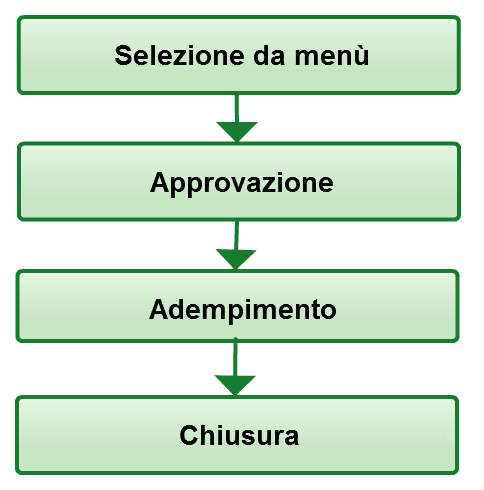
\includegraphics[scale=0.4]{Images/Diagrams/Request_fulfillment.png}
\caption{Flusso attività del processo di \ac{Request-Fulfillment}}
\label{rf-flow-img}
\end{figure}

\begin{center}
\begin{longtable}{| p{3cm} | p{2cm} | p {7cm} |}
\caption{Elenco attività di processo}
\label{rf-flow-table}\\
\hline
\multicolumn{1}{| c |}{\textbf{Ruolo}} & \multicolumn{1}{| c |}{\textbf{Step}} & \multicolumn{1}{| c |}{\textbf{Descrizione}}\\
\hline
\endfirsthead
\hline
\multicolumn{1}{| c |}{\textbf{Ruolo}} & \multicolumn{1}{| c |}{\textbf{Step}} & \multicolumn{1}{| c |}{\textbf{Descrizione}}\\
\hline
\endhead
Utente & 1 & L'utente invia una richiesta di servizio presso il \english{Service Desk} dell'\entity{}. La richiesta avviene tramite l'apertura di un \english{ticket}.\\
\hline
\multirow{6}{*}{Staff tecnico} & 2 & Determinare se si tratta di una richiesta pre-approvata (\ac{assistance-Service-Request}). Se si tratta di questo tipo di richiesta seguire quanto riportato nel documento associato, altrimenti proseguire con il passo 3.\\
\cline{2-3}
& 3 & Determinare se si tratta di un incidente. Se si tratta di un incidente passare la richiesta al processo di \ac{Incident-Management}, altrimenti procedere con il passo 4.\\
\cline{2-3}
& 4 & Eseguire una analisi di fattibilità e se la richiesta è approvata risolverla.\\
\cline{2-3}
& 5 & Notificare l'utente a seguito della risoluzione oppure delle motivazioni per cui non è risolvibile.\\
\cline{2-3}
& 6 & Richiedere conferma di soddisfazione da parte dell'utente. Se l'utente è soddisfatto procedere con il passo 7 altrimenti ritornare al passo 5.\\
\cline{2-3}
& 7 & Chiudere la richiesta completando la relativa documentazione.\\
\hline
\end{longtable}
\end{center}